
\section{Высшее образование и аспекты релятивности работников}
Профессия медицинская физика пользовалась успехом на протяжении многих десятилетий, в результате возникшего интеллектуального разнообразия подхода обучения -- для многих физиков до начала нынешнего века их образование было докторской степенью по физике вместе с обучением на рабочем месте и самоподготовкой по медицинской физике.  Однако, компетентность и готовность медицинских физиков к выполнению клинической работы были весьма сомнительны. 

Сегодня пути к тому, чтобы стать квалифицированным (клиническим) медицинским физиком, четко определены и стандартизированы согласно рекомендациям МКРЗ. Рис.\ref{ed} показывает траектории обучения, начинающиеся с получения степени бакалавра по физике (или равнозначимой смежной области) и заканчивающиеся получением начального уровня в данной специальности.
Согласно AAPM, квалифицированный медицинский физик сможет получить степень магистра и/или доктора в области физики, медицинской физики, биофизики, радиологической физики, медицинской физики здоровья или равнозначимых дисциплин в аккредитованном колледже/университете. Кроме того, квалификация требует сертификации в конкретной области медицинской физики, соответствующим национальным органом по сертификации и соблюдения текущих требований к непрерывному образованию \cite{AAPM 2016b}. 

Так устроено образование за рубежом. В РБ с образованием ситуация такова: Минский государственный экологический институт имени Андрея Дмитриевича Сахарова при Белорусском государственном университете выпускает с 2018 года студентов по специальности <<медицинский физик>>. Затем следует поступление на магистратуру, после чего -- заступление на рабочее место по обслуживанию ускорителей, по разработке и внедрению приспособлений технологий для обеспечения качества диагностических и терапевтических процедур, занимается организаторской работой по разъяснению работникам организации здравоохранения вопросов обеспечения безопасности пациентов и работников. И, вроде бы, образовательные стандарты исполняются, внедряются необходимые мероприятия и директивы. Но ожидания не оправдываются -- неопределенности во вхождении в штат больниц, обязанностей специалиста, неоднозначность в получаемой профессии, исходящая из разрыва между преподаваемыми в высшем учреждении теоретическими положениями и практической деятельностью. 

Переходя за <<границу>>, кадровые проблемы сложны и будущее рабочей силы неопределенно. Факторы которых, являются высокий рост заболеваемости раком и приблизительно соответствующие возможности учебных программ. Несостоятельности предостаточно -- влияние изменений здравоохранения (экономической), использование радиации в медицине, эффективность процедур медицинской физики и форма надвигающейся волны отставок. По этим причинам тенденции спроса и предложения трудно предсказать более чем на несколько лет вперед. Таким образом, в настоящее время неизвестно, будет ли медицинский физический персонал адекватным через несколько лет \cite{Newhauser}. 
 
%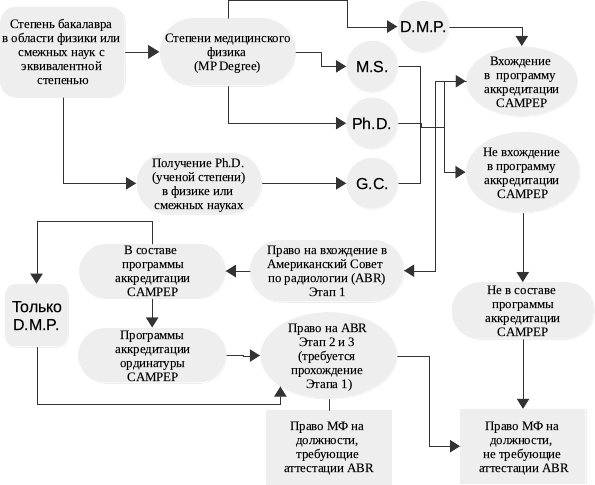
\includegraphics{edpath} \\ {Рис.1 -- }{Внутренние и внешние связи подсистемы управления услугами}




%\begin{table}
%\caption{Пример таблицы}
%\centering
%\begin{tabular}{llr}
%\toprule
%\multicolumn{2}{c}{Name} \\
%\cmidrule(r){1-2}
%First name & Last Name & Grade \\
%\midrule
%John & Doe & $7.5$ \\
%Richard & Miles & $2$ \\
%\bottomrule
%\end{tabular}
%\end{table}

%\blindtext % Dummy text
%
%\begin{equation}
%\label{eq:emc}
%\frac{dp}{dt}=\vec{F}
%\end{equation}

%\blindtext % Dummy text

%------------------------------------------------




%\subsection{}



%A statement requiring citation \cite{No174}.
%\blindtext % Dummy text

%\subsection{}

%\blindtext % Dummy text
%------------------------------------------------
